\documentclass{article}
\usepackage{amsmath, amssymb, graphicx}

\title{Economics 101: Problem Set Solutions}
\author{Your Name}
\date{\today}

\begin{document}
\maketitle

\section*{Part I: Multiple Choice and Short Answer}

\subsection*{1. Marginal Opportunity Cost Calculation}

Given the production possibilities table:

\begin{center}
    \begin{tabular}{|c|c|c|}
        \hline
        Point & Machines & Food \\
        \hline
        A & 0 & 50 \\
        B & 2 & 45 \\
        C & 4 & 38 \\
        D & 6 & 28 \\
        E & 8 & 15 \\
        F & 10 & 0 \\
        \hline
    \end{tabular}
\end{center}

To move from B to C:

\[
\text{Marginal Opportunity Cost} = \frac{\text{Lost Food}}{\text{Gained Machines}} = \frac{45 - 38}{4 - 2} = \frac{7}{2} = 3.5 \text{ food units per machine}
\]

\textbf{Answer:} 3.5 units of food per machine.

\subsection*{2. Manuel's Decision to Run One More Mile}

Manuel's decision implies that the \textbf{marginal benefit} of running exceeded the \textbf{marginal cost}. 

\textbf{Correct answer:} B) The marginal benefit outweighed the cost.

\subsection*{3. Cuba's Economic Decline}

Cuba lost economic support, reducing its productive capacity. This causes an \textbf{inward shift} in the production possibilities curve.

\textbf{Correct answer:} B) Inward shift of the PPC.

\subsection*{4. Opportunity Cost Concept}

The best phrase to describe opportunity cost is:

\textbf{Correct answer:} C) "There is no such thing as a free lunch."

\subsection*{5. Unemployment and the PPC}

Unemployment means not all resources are used efficiently, placing the economy \textbf{inside} the PPC.

\textbf{Correct answer:} D) Point inside the PPC.

\subsection*{6. Tuition and Enrollment at GSU}

If tuition and enrollment have both risen, demand must have increased due to factors like population growth or preferences.

\textbf{Correct answer:} C) Demand increased due to population, income, or preference changes.

\subsection*{7. Optimal Output of Shoes}

The optimal output level is where \textbf{marginal cost = marginal benefit}, occurring at $Q_2$.

\textbf{Correct answer:} B) $Q_2$.

\section*{Part II: Short Essay}

\subsection*{1. Equilibrium Price and Quantity Changes}

\textbf{(A) Hot Day: Increase in Both Demand and Supply of Lemonade}
\begin{itemize}
    \item \textbf{Demand shifts right} (more people want lemonade).
    \item \textbf{Supply shifts right} (more lemonade is produced).
    \item \textbf{Price: Indeterminate} (?).
    \item \textbf{Quantity: Increases}.
\end{itemize}

\textbf{(B) Hawaii Volcano Eruption: Increased Demand, Decreased Supply}
\begin{itemize}
    \item \textbf{Demand shifts right} (tourists want flights).
    \item \textbf{Supply shifts left} (fewer pilots willing to fly).
    \item \textbf{Price: Increases}.
    \item \textbf{Quantity: Indeterminate} (?).
\end{itemize}

\textbf{(C) Windy Day in Arizona: Demand Decreases, Supply Increases}
\begin{itemize}
    \item \textbf{Demand shifts left} (less AC use).
    \item \textbf{Supply shifts right} (more electricity from wind).
    \item \textbf{Price: Decreases}.
    \item \textbf{Quantity: Indeterminate} (?).
\end{itemize}

\textbf{(D) Decline in Cycling Interest in Italy}
\begin{itemize}
    \item \textbf{Demand shifts left} (fewer cyclists).
    \item \textbf{Supply shifts right} (new technology lowers costs).
    \item \textbf{Price: Decreases}.
    \item \textbf{Quantity: Indeterminate} (?).
\end{itemize}

\subsection*{2. Optimal Production Technique}

Given the following costs:

\begin{center}
    \begin{tabular}{|c|c|c|c|c|}
        \hline
        Technique & Labor Cost & Land Cost & Capital Cost & Total Cost \\
        \hline
        A & 4 × \$10 = \$40 & 10 × \$5 = \$50 & 5 × \$15 = \$75 & \textbf{\$165} \\
        B & 5 × \$10 = \$50 & 3 × \$5 = \$15 & 3 × \$15 = \$45 & \textbf{\$110} \\
        C & 5 × \$10 = \$50 & 2 × \$5 = \$10 & 4 × \$15 = \$60 & \textbf{\$120} \\
        \hline
    \end{tabular}
\end{center}

\textbf{Best choice:} Technique B (\$110, lowest cost).

\[
\text{Profit} = 135 - 110 = 25
\]

Since there's a profit, the industry will expand until competition reduces profits.

\subsection*{3. Overproduction of Good X}

If marginal cost exceeds marginal benefit, society is producing \textbf{too much} of Good X.

\section*{Part III: Long Essay (Impact of Sustainable Fashion)}

\subsection*{(A) Price and Quantity of Sustainable Clothing}
- Increase in supply leads to \textbf{lower prices, higher quantity}.
- \textbf{Graph: Rightward shift in supply curve.}

\subsection*{(B) Price and Quantity of Fast Fashion}
- Decrease in demand leads to \textbf{lower prices, lower quantity}.
- \textbf{Graph: Leftward shift in demand curve.}

\subsection*{(C) Price of Clothing Accessories}
- Increase in demand leads to \textbf{higher prices, higher quantity}.
- \textbf{Graph: Rightward shift in demand curve.}

\begin{figure}[h]
    \centering
    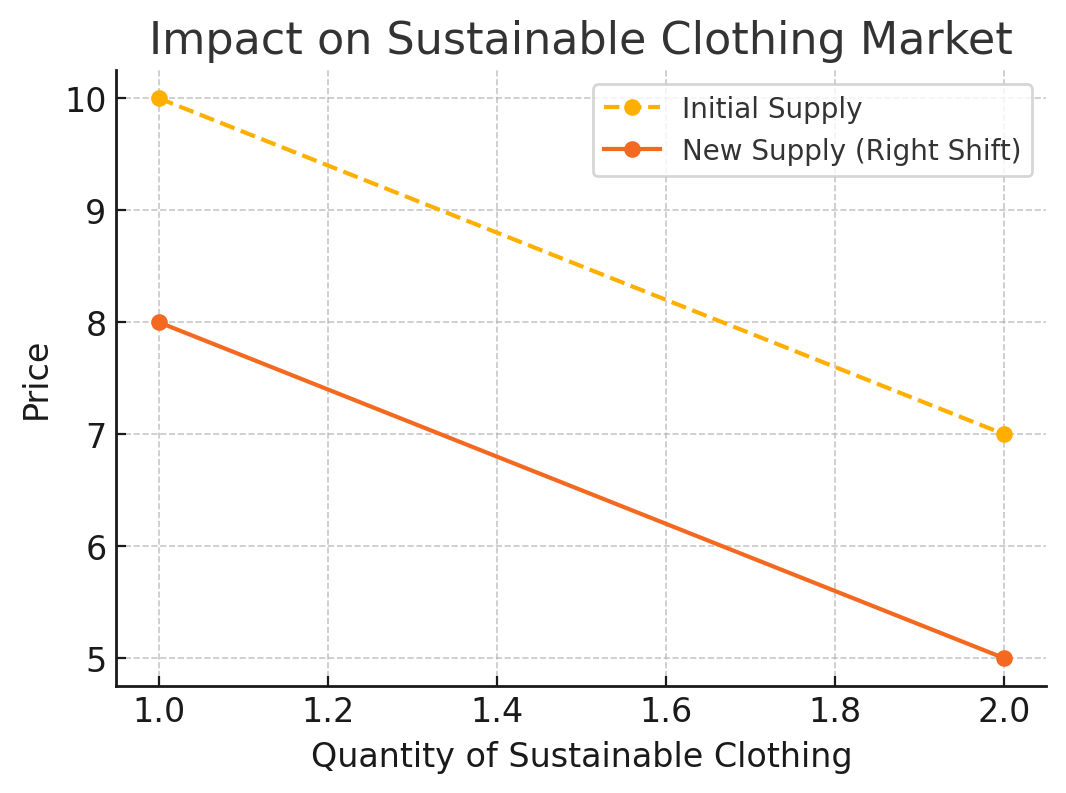
\includegraphics[width=0.4\textwidth]{Photos/ImpactOnSustainableClothingMarket.png}
    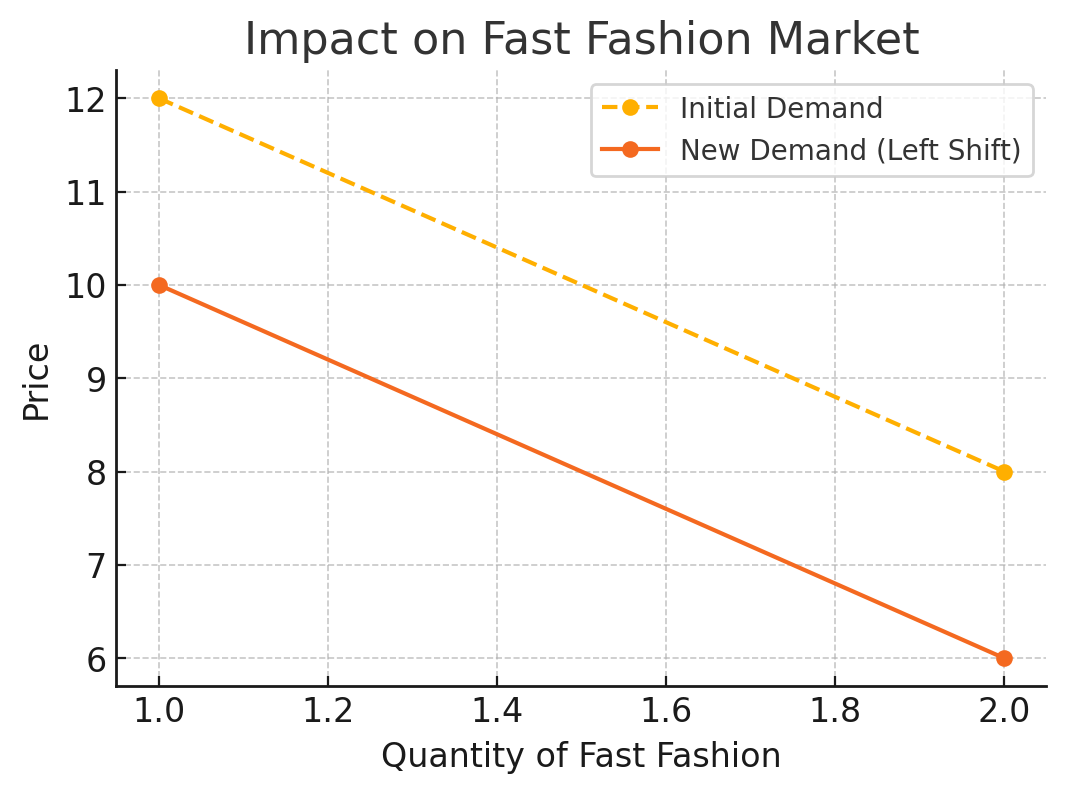
\includegraphics[width=0.4\textwidth]{Photos/ImpactOnFastFashionMarket.png}
    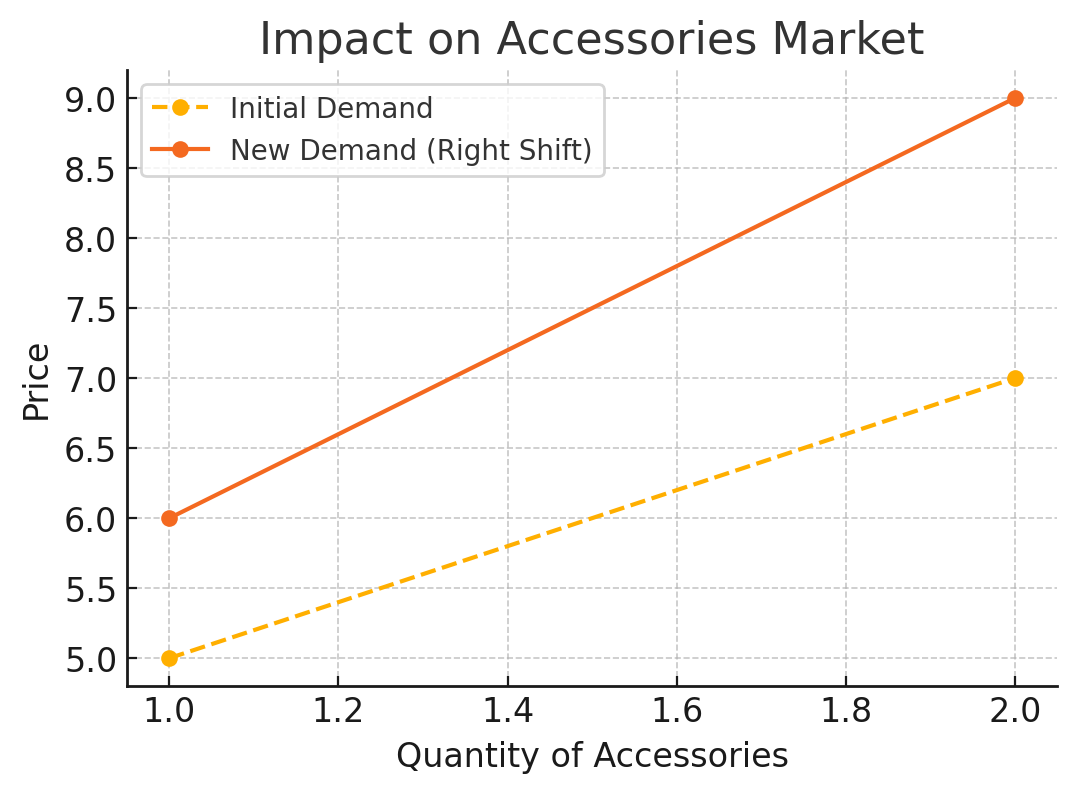
\includegraphics[width=0.4\textwidth]{Photos/ImpactOnAccessoriesMarket.png}
    \caption{Graphs showing market changes.}
\end{figure}

\end{document}
